%% This is an example first chapter.  You should put chapter/appendix that you
%% write into a separate file, and add a line \include{yourfilename} to
%% main.tex, where `yourfilename.tex' is the name of the chapter/appendix file.
%% You can process specific files by typing their names in at the 
%% \files=
%% prompt when you run the file main.tex through LaTeX.
\chapter{Motivation and Background}

\begin{flushright}
\textit{``The mathematician�s patterns, like the painter�s or the poet�s 
must be beautiful; the ideas like the colours or the words, must fit 
together in a harmonious way. Beauty is the first test: there is no 
permanent place in the world for ugly mathematics."
}
G. H. Hardy \cite{hardy}
\end{flushright}


In order to illustrate the unique creative potential algorithmic craft, it is useful to first examine its components independently.  Computational design, digital fabrication and traditional craft all have qualities that facilitate specific forms of creation. Because they are both digital mediums, digital fabrication and computational design possess a set of shared qualities that allow them to work well together. The differences between craft and computation are more severe and often put these two mediums at odds with one another. The techniques and processes of craft are directly informed by specific material properties. Computation on the other hand is defined by its abstraction. With appropriate programing, a computer can embody any conceivable process \cite{mateas}.  Digital fabrication  they can be combined through the bridge of digital fabrication. Each of these disciplines have separate strengths and limitations. Through their convergence in algorithmc craft, it is possible to apply these strengths to new spaces, and overcome many of their limitations. 

\section{Computational Design}\label{sec:computational_design}
The practice of computational design is different from contemporary design. Due to the variety of  approaches among different designers, it is difficult to describe a standard design process however it is useful to describe the key features of computational design that stand in contrast with the conventional design.

Both computational and conventional designers begin with a design problem. Conventional designers often proceed by roughing out a number of specific solutions to this problem. These early solutions are evaluated against one another for their successes and drawbacks. From this evaluation a smaller set of more refined solutions are produced. This iterative process may continue, until a single solution is reached that is sufficiently refined and successful in addressing the initial problem. 
Computational design incorporates many of the iterative principles of conventional design, but differs significantly in its approach. Rather than begin by developing a concrete solution to the initial design problem problem, the computational designer must first formalize the elements of the  problem into a set of rules. The designer then creates a system based on these rules which is capable producing a variety of solutions. In its simplest form, this system may consist of a single algorithm with static input and limited output  solutions. More frequently however, the computational design process produces complex systems that act on upon a wide range of input criteria and parameters, and can produce nearly infinite number of design solutions. Iteration in computational design often takes the form of making adjustments to the system. By sampling a number of outputs from a system, the designer can "tweak" or make adjustments to the rules that govern the system, eventually resulting in more and more desirable output solutions. This process of sampling and tweaking is continued until the designer is satisfied with a given range of outputs. The designer can then vary the input to the system and can select among the resulting solutions. 
 
 Computational design is compatible with conventional design techniques, and can also be considered as a means of extending traditional design practice through several key affordances: These include the following:
\begin{itemize}
\item \textbf{Precision:} Computation supports high levels of numerical precision with relatively little effort on the part of the designer.
\item \textbf{Automation:}  Computation allows for rapid automation of repetitive tasks. Automation often plays a key role in enabling the development and transformation of complex patterns and structures, through the combination of large numbers of simple elements in an ordered and structured manner.
\item \textbf{Generativity and randomness:} Computation allows for the programmer to create algorithms which when run, allow for the computer to autonomously produce unique and often unexpected designs.
\item  \textbf{Parameterization:} Computation allows users to specify a set of degrees of freedom and constraints of a model and then adjust the values of the degrees of freedom while maintaining the constraints of the original model \cite{reas}.
\item \textbf{Documentation and remixing:} Computationally generated designs are generated by a program, which can be shared with and modified by other designers. Because these programs are often text-based, they also serve as a form of documentation of the design process. 
\end{itemize}	

In combination with these affordances however, computational design also incorporates  a number of challenges in the design process that are not present in traditional design:
\begin{itemize}
\item \textbf{Formalizing complex problems} As design problems grow in complexity, formalizing the problem in a manner that can be expressed programmatically becomes challenging. Writing an algorithm to generate a visual pattern is simple, however writing a program to incorporate that pattern into the design of an entire garment  is difficult. 
\item \textbf{Creating singularities:} A designer will often choose to deviate from a set pattern or structure at specific points in order to create a special emphasis in that area. Because computational design is governed by a systematized ruleset, the methods of breaking these rules at arbitrary points is are often unclear and tedious to implement. 
\item \textbf{Selecting a final design:}  The systematic approach to computational design gives the designer the ability to produce extremely large numbers of solutions to a single design problem. While this is useful in situations where multiple solutions are required, when a single design must be chosen, the process of deciding on a solution is often difficult and sometimes arbitrary, especially if the decision is based on aesthetic criteria.
\end{itemize}

\section{Digital Fabrication} Although computational design must be conducted on a computer to some degree, the artifacts generated by computational design are not restricted to the screen. Digital fabrication  technology provides the opportunity to translate digital files to physical form, and can act as a conversion point between a programmatically generated design and an actual object based on that design. 

Digital Fabrication is the process of using computer-controlled machines to fabricate objects specified by a digital tool path.  Digital fabrication shares many of the affordances of computational design. In particular, it allows for the creation of physical objects of great complexity without formal skill in craft or extensive manual labor. Digital fabrication also allows for the rapid production of small volumes of similar or identical objects. Lastly, because the artifacts produced through digital fabrication are derived from digital files, anyone with access to the file, and a similar fabrication machine can create a copy of the object, or incorporate elements of it into a new design. 

There are two primary forms of digital-fabrication manufacturing, additive and subtractive. Subtractive processes machine a part by removing pieces from the original material and include tools like laser cutters, computer numerically controlled (CNC) milling machines and vinyl cutters. Additive  processes create a part by incrementally adding successive layers of material. 3D printers are most commonly associated with additive manufacturing, however  ink jet printers and CNC embroidery machines also fit this definition. Additive technology is newer than that of subtractive and still fairly restrictive. Although it is changing, 3D printers are limited to a few forms of plastic, ceramic and metal composites. Low-end 3D printers are even more limited, generally to one form of ABS plastic. The price of Additive manufacturing increases steeply with increases in scale. 

 Subtractive processes on the other hand, make it possible to work at a much larger scale than additive processes for a much lower price, and can work with a wide range of materials.  Laser cutters work well with traditional materials such as  wood, paper and cloth. Vinyl cutters can also be used on cloth and paper, as well as cut vinyl patterns which can be used for screen printing. Milling machines can cut parts from a variety of plastics, foams and wood. In specialized cases these machines can also be modified to function in an additive manner with custom attachments. An example is the adaptation of a 3-Axis ShopBot by machine to function as a threading device to facilitate part of the construction of a Silk Pavilion, created by the Mediated Matter Group at MIT (figure \ref{fig:pavilion} \cite{pavilion}.)  

\begin{center}
\begin{figure}[h!]
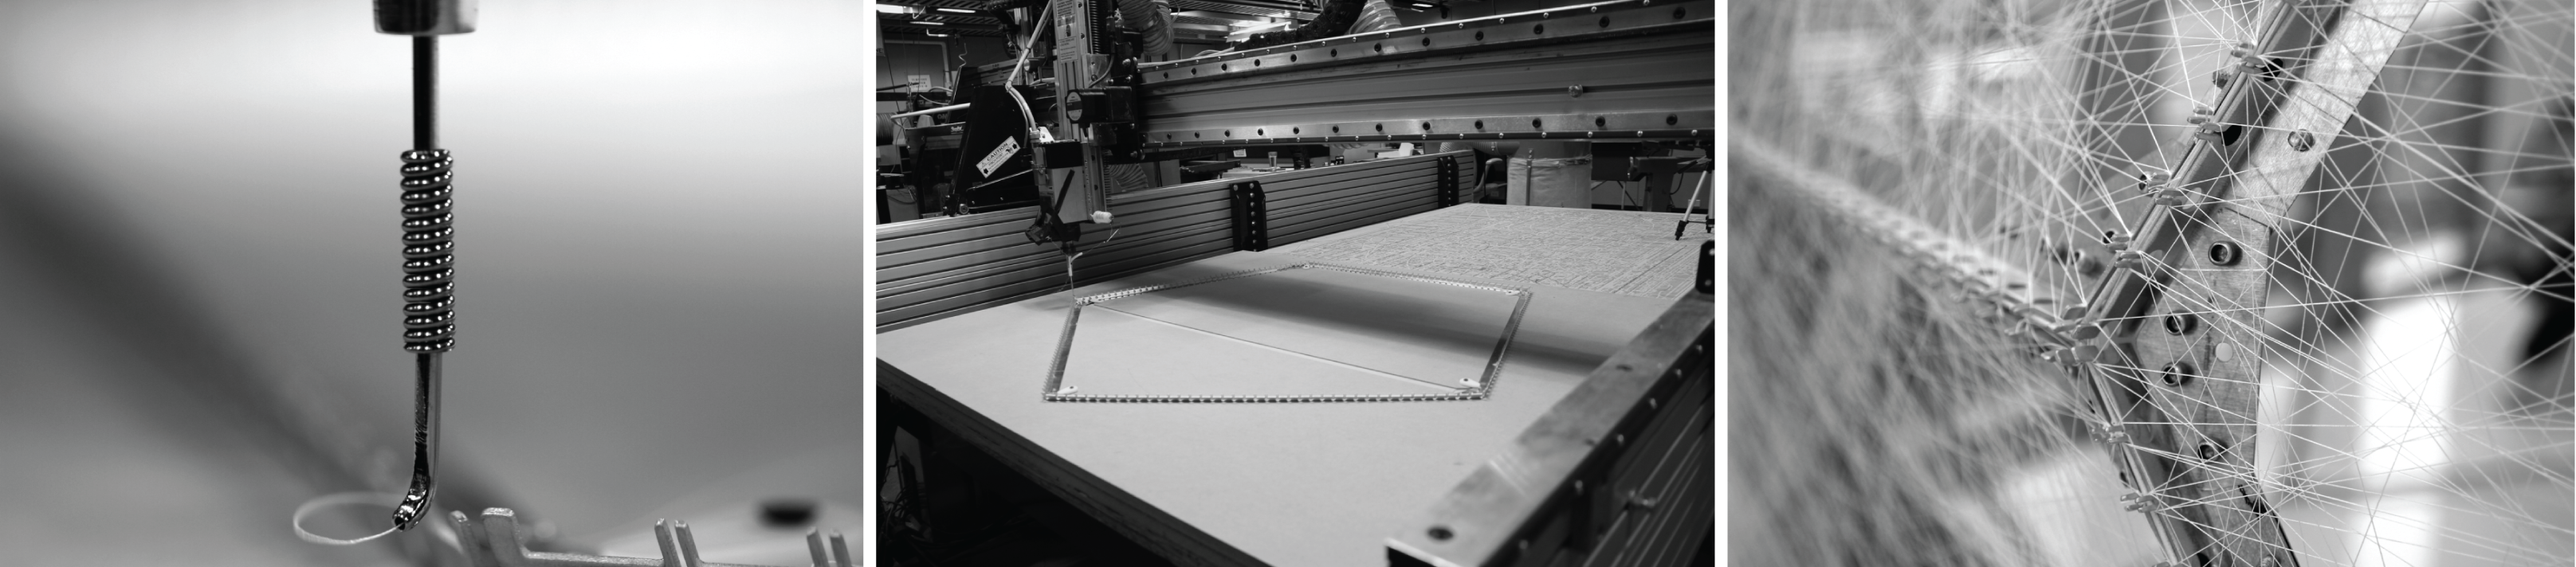
\includegraphics[width=\columnwidth]{images/pavillion_shopbot.png}
\caption{3-axis CNC milling machine adapted as CNC deposition tool using a custom threading tool. (Part of the Silk Pavilion Fabrication process)}
\label{fig:pavilion}
\end{figure}
\end{center}

Currently, digital fabrication machines are rapidly decreasing in price and increasing in availability \cite{gershenfeld}. The trend of personal fabrication allows individuals and small groups to have access to  sophisticated manufacturing technologies \cite{lipson}. Consumer 3d printers can now be purchased at prices ranging from \$1,000-\$3,500 dollars. Small scale laser cutters and milling machines are available at prices ranging from \$3,000 to \$5,000. \todo{add in citations for prices} In addition, other groups are producing open-source versions of commercial fabrication equipment, like the MTM snap CNC milling machine, the LaserSaur laser cutter and the RepRap 3d printer. Though these devices require additional levels of expertise to assemble, they point to to exciting future developments in the range and accessibility of these machines. Though often dismissed, machines like inkjet printers and craft cnc vinyl cutters also function as personal fabrication devices and are extremely accessible and affordable. 

There are also options for individuals without direct ownership of a fabrication machine. Community hacker spaces like Artisans' Asylum in Cambridge, NYC resistor in New York and Noisebridge in San Francisco, and organizations like the FabLab network provide access to shared digital fabrication facilities.  Online services like Shapeways, Ponoko and SpoonFlower offer on-demand fabrication services to individual consumers for a variety of materials and machining processes. Although the current stage of personal fabrication still contains many limitations, it signals a societal shift in how individuals and small groups have access to the means of production.

\section{Algorithmic Craft}
The connotations of craft have varied throughout history, but several key elements have remained consistent.  Primarily craft refers to the production of artifacts through the use of one�s hands {\cite{craft_reader}}. Craft is also defined by its connection to the material world, wherein interaction with the raw materials informs the production of the work. Because digital fabrication machines produce physical artifacts, they offer a transition point between the digital world of computation and the material world of art and craft. 

Subtractive technologies in particular can work with materials often used in traditional forms of craft. For example, laser cutters work well with wood, paper and cloth. Vinyl cutters can also be used on cloth and paper, as well as cut vinyl patterns which can be used for screen printing. Materials like wood, paper and fabric also have the property of being highly mutable following the fabrication process, through sanding, hand-cutting, sewing and folding. The merging of computational design, digital fabrication and crafting allows for a creative practice that exhibits the variability and complexity of computation, the precision and repeatability of fabrication and the material concerns and felt knowledge of craft. Algorithmic crafting therefore, provides opportunities for new forms of artifact production, and allows individuals use programing and digital fabrication as a means of pleasurable and useful creative expression. In addition, algorithmic craft suggests the incorporation of  the approaches and values of artisans and craftspeople in development of new methods of digital fabrication and computational design tools, paving the way for new forms of innovation in these fields. 

\todo{Cite Amit Zoran and Peter Schmitt's work here... algorithmic quilt and others?}

\section{Challenges in broad participation in computational design and digital fabrication}
Despite the opportunity for casual, non-professional engagement in computational design and digital fabrication, this domain is largely limited to experts and professionals.  Novice practitioners in this field are confronted with the difficult process of translating their code-based design to a format that is compatible with the target fabrication machine. Furthermore, the challenges involved in designing complex objects from multiple digitally fabricated parts are extremely difficult to tackle for casual users. There are also severe limitations on computational design software for novices capable of supporting digital fabrication. The majority of traditional CAD tools do not contain computational design capabilities intended for novice use. Similarly, novice oriented programing environments lack the functionality to allow the production of designs that are suitable for fabrication. 

There are also significant perceptual barriers to participation. There persists among the general public a  limited perception of the applications of programing. Many people consider programing to be irrelevant to their interests, and therefore lack motivation to pursue what they perceive to be a highly specialized and difficult undertaking [12]. There are also prevailing perceptions of digital fabrication which may hinder casual engagement. Personal fabrication technology is often portrayed as a precursor to the production of replicator-like technology which can instantiate literally anything by building it directly from atoms. This projection of future technology is exciting to think about. This view can also act as a barrier to widespread engagement with existing forms of digital fabrication, by setting up unreal expectations for this technology,or by portraying it as a variation on traditional forms of consumerism. The idea of fabrication as a perfect replication system also eliminates the need or desire for human engagement in the fabrication process, eliminating the entry points for craft. Daniella Rosner describes this view in her research:

\begin{flushright}
 \textit{A central element of these and  other visions of the future is that  craft is done for us: Kitchens tell us what and how to cook, eliminating the creativity and pleasure of  cooking from scratch with what�s on hand; object printers create flawless prototypes, eliminating messily glued-together chipboard and toothpicks. In this new 
world, craft becomes fetish�the proudly displayed collection of vinyl records shelved alongside an iPod and digital files \cite{rosner_craft_vs_design}.}
\end{flushright}

There is also the tendency to trivialize the hobbyist applications of digital fabrication. In the domain of Human Computer Interaction (HCI), researchers often focus on the hedonistic properties technologically oriented DIY practices as opposed to the utility  of the resultant artifacts or their ability to generate profit. Pleasure and self-expression are central components of hobbyist  and craft-oriented computation and digital fabrication, however these qualities do not come at the cost of generating artifacts that are practical, functional, and sellable \cite{tanenbaum}. The trend of separating hobbyist practice as merely fun in contrast to professional practical applications overshadows some of the most interesting practical possibilities that emerge through amateur use of this technology. 


